\subsection{The APEX Approach}
\begin{figure}[!t]
	\includegraphics[width=\columnwidth]{figures/tool_single.png}
	\caption{One step in the APEX tool: the local planner generates a trajectory, which is automatically input into the mission description file and verified using dReach}
	\vspace{-10pt}
	\label{fig:apexsingle}
\end{figure}

 \begin{figure*}[!t]
 	\centering
 	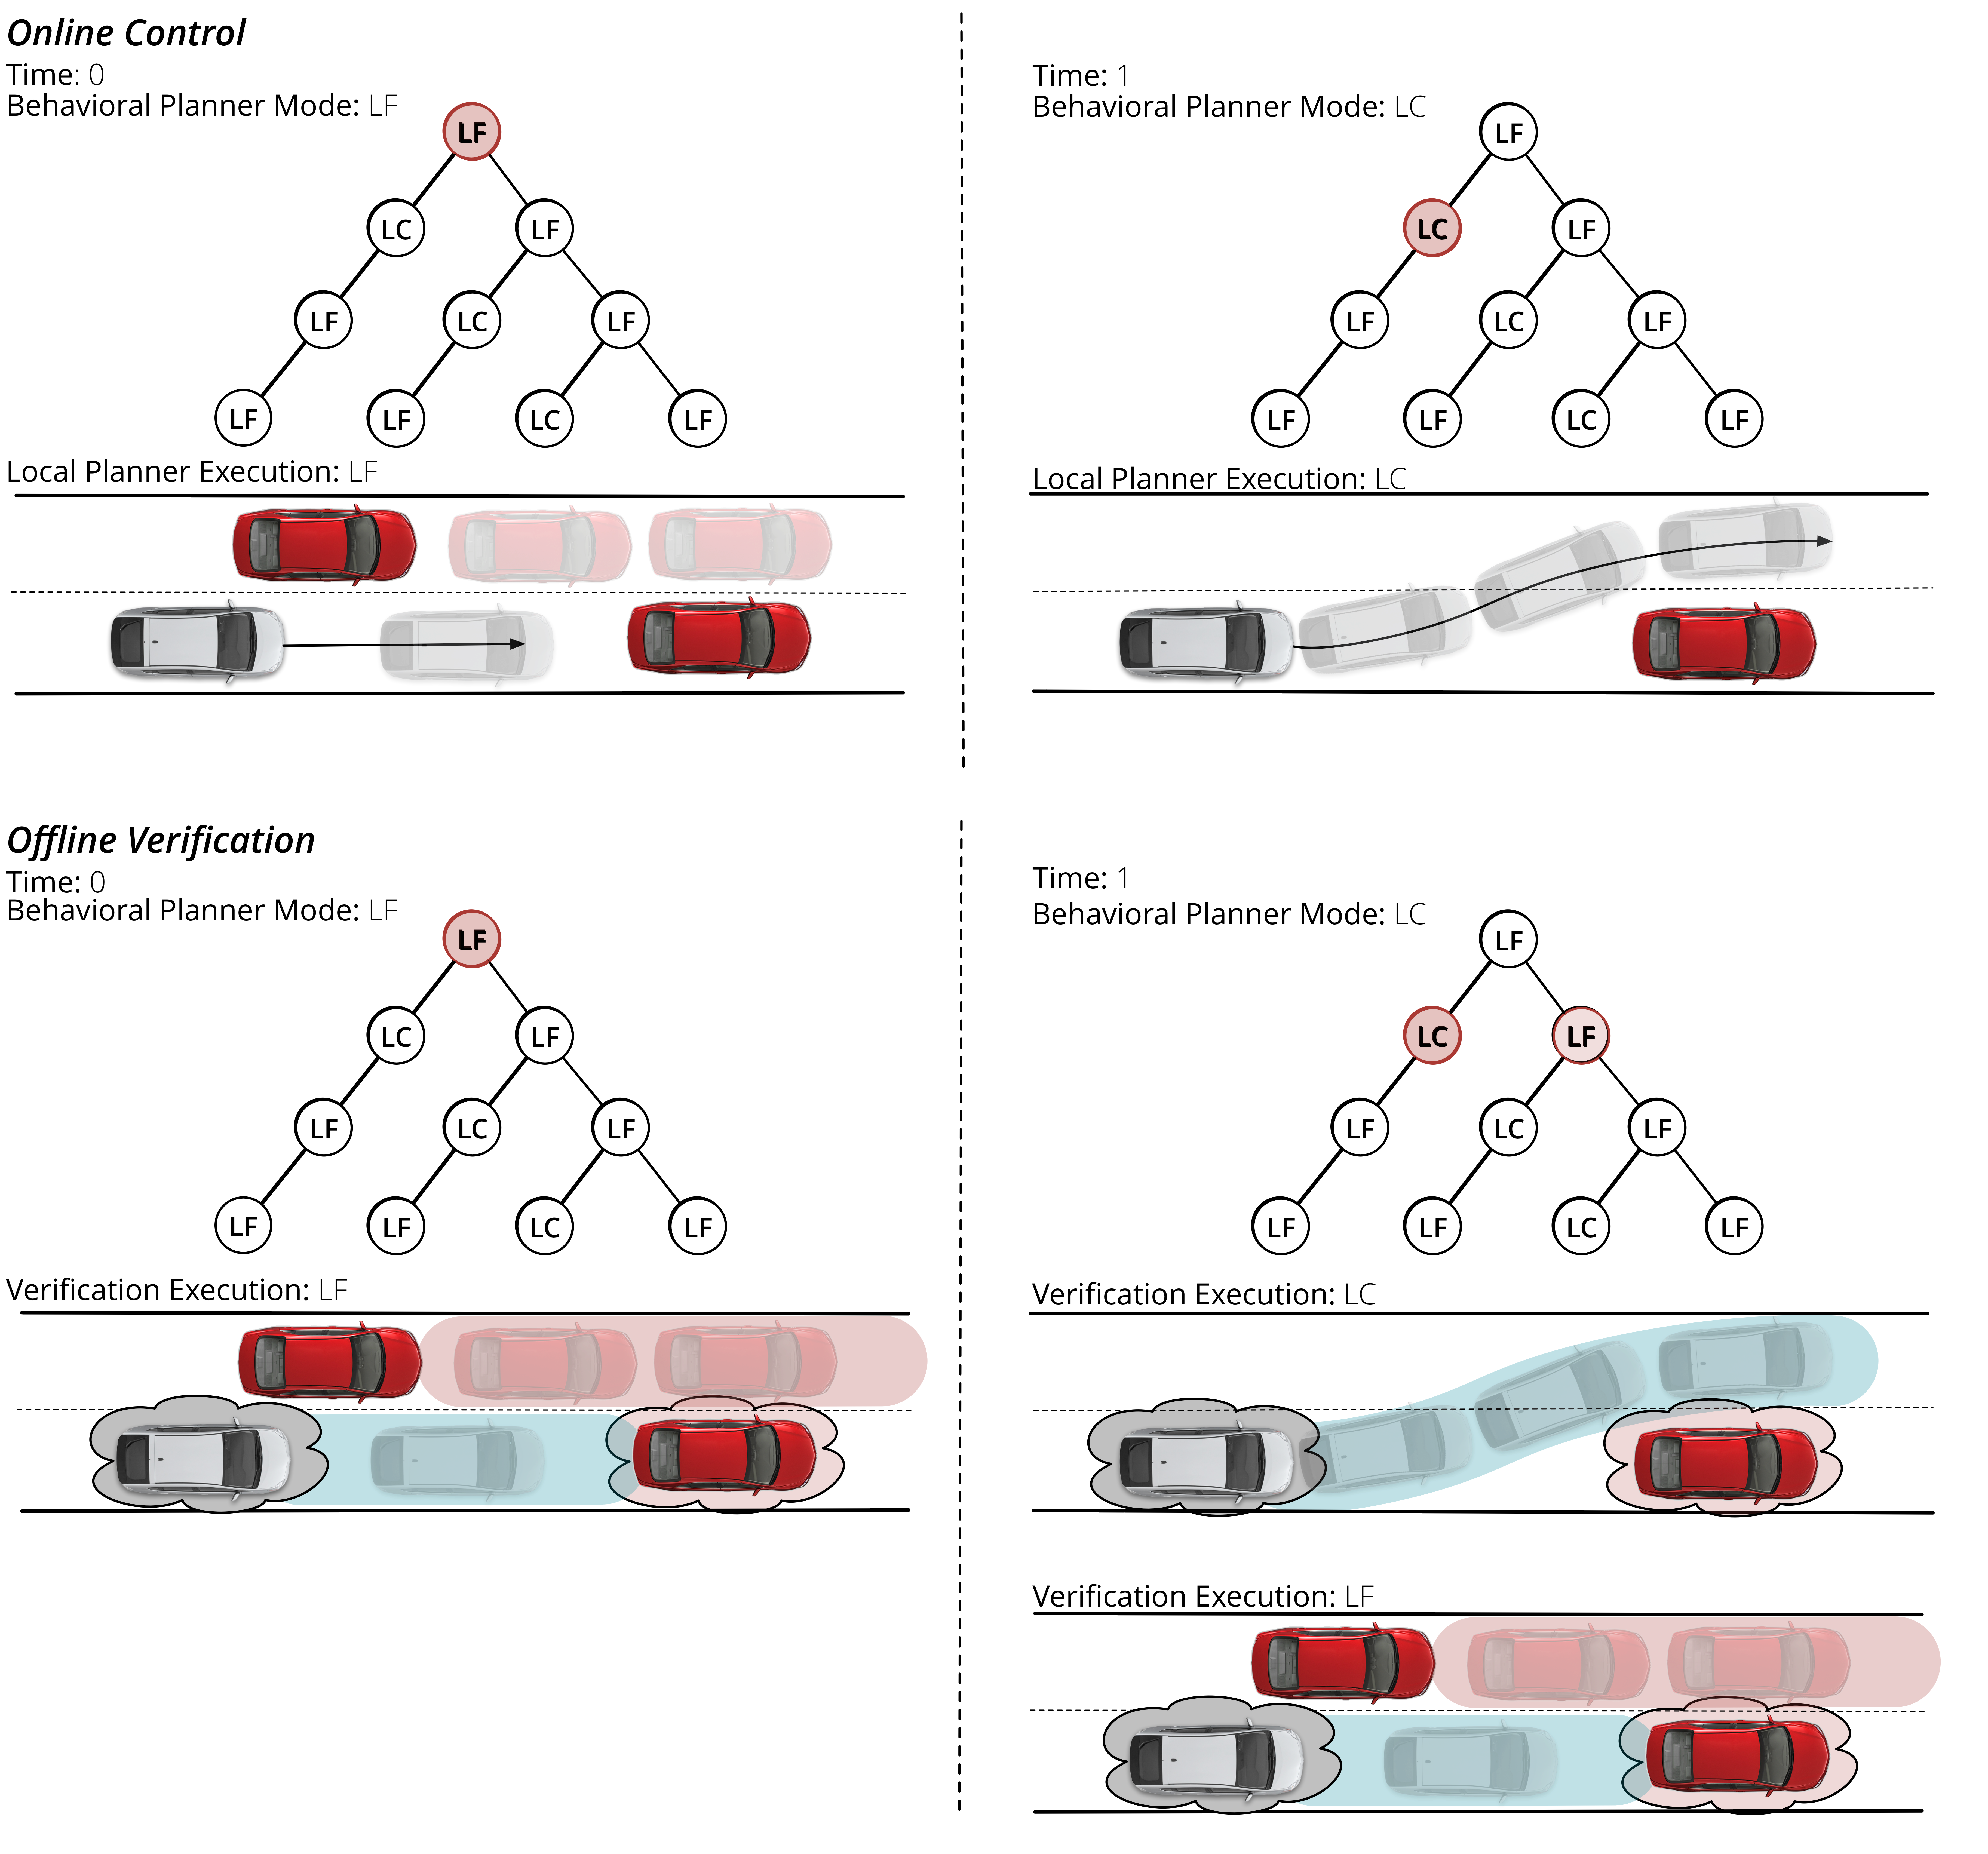
\includegraphics[width=\textwidth]{figures/apex_approach.pdf}
 	\caption{ \small Stages of APEX verification and their correspondence to control execution. Top left: at $t=0$, mode is Lane Follow (LF) and the vehicle follows the current lane. Top right: at $t=1$, mode is Lane Change (LC) and vehicle starts a lane change maneuver. Bottom left: offline, APEX verifies that in mode LF, the vehicle can track the trajectory. Bottom right: offline, APEX verifies both possible executions, a lane change and a lane following.}
	\vspace{-10pt}
 	\label{fig:apex_internals}
 \end{figure*}
APEX answers the following question by re-formulating it as a reachability problem: given some initial uncertainty about the state of the AV, constraints on the configuration of the environment, and a desired behavior of the AV (like mobility goal and traffic laws), is it ever possible for the AV to violate the desired behavior?
Fig. \ref{fig:apexsingle} summarizes a single execution of the verification engine.
For each trajectory selected by the planner (highlighted in red), APEX calls dReach~\cite{gao2014delta}, a reachability analysis tool for nonlinear hybrid systems.
% 
%The APEX approach to formal verification of AVs and ADAS systems seeks to follow plan executions through to the vehicle's actual motion in the environment rather than exploring abstract motion on a grid.

We emphasize that the verification process is \emph{offline} - the vehicle does \emph{not} run APEX while it is driving.
At each decision point encountered by the behavioral planner there may be multiple executions of the verification engine depending on the design of the behavioral planner. Fig. \ref{fig:apex_internals} describes how the execution of the controller online relates to the \emph{offline} verification process. In contrast to the simulation based approach outlined in the introduction, the result of the APEX approach is that we have converted a brute force search over real intervals into a finite series of tractable bounded reachability problems over a finite verification horizon.
% In certain cases we may even deduce infinite time system properties via an investigation of a finite number of reachability problems. 

\subsection{Tool Input}
APEX is a \emph{command line tool} for verification of autonomous vehicle missions written in Python and C++.
The input to the verification process is a \emph{mission definition file}. 
The \emph{mission definition file} defines the sequence of waypoints or road links which the vehicle will traverse in order to achieve a mobility goal. 

The \emph{mission defintion file} describes the following:
\begin{itemize}
	\item \emph{The collection of agents in the scenario}, consisting of the ego vehicle and other cars in the scenario.
	The agents are described via ODEs that describe the evolution of their state with time, and their behavioral planners, which give the next waypoints for each vehicle.
	All agents operate in an ontology specific to the mission, in this case the world model consists of a geometric description of a road network. 
	\item \emph{Set of initial states} for each state variable of every vehicle.
	\item \emph{The constraints that the AV should satisfy}, such as traffic laws and the unsafe conditions that ego vehicle must avoid. These are described in MITL. 
	\item \emph{The goal of the ego vehicle}, also expressed in MITL \cite{alur1996benefits}. 
\end{itemize}

The mission definition file is part of a \emph{mission definition script}.
The latter manages the execution of the behavioral planner and trajectory generator.
Each (state, goal) pair that is encountered on the mission generates at least one trajectory which must be verified. The \emph{mission definition script} automatically updates a \emph{scenario verification instance}. The \emph{scenario verification instance} is a dReach (.drh) file which combines the results of the plan execution with the dynamical model of the vehicle and a low-level trajectory tracking controller. The \emph{agent definition file} contains the dynamical model of the vehicle and the tracking controller is also written using the syntax of dReach, it may be manually edited in order to match mission specific vehicle models. We provide an example of the syntax of the composed \emph{scenario verification instance} in Fig. \ref{fig:scenario_ver}.


Together, the constraints of the environment $\xi$ and ego vehicle goal and constraints $\phi$ constitute the \emph{specification} of the mission.
The mission is a success if every execution of the system (i.e., every simulation) satisfies the specification.
%We stress, however, that we are \emph{not} simulating the scenario. 
%Rather the formal verification approach we use allows us to make assertions about every execution of the system without actually simulating it.

\begin{figure}[!t]
	\centering
	\includegraphics[width=\columnwidth]{figures/code}
	\caption{Scenario verification instance generated by APEX}
	\label{fig:scenario_ver}
\end{figure}

\subsection{Tool Output}
Each \emph{scenario verification instance} can  return either SAFE or $\delta$-UNSAFE. SAFE means that for all possible executions of the system we can not reach an unsafe state.
$\delta$-UNSAFE means that there exists an execution of the system which comes within a $\delta$ of the unsafe region, and possibly enters it. If the system is $\delta$-UNSAFE the tool will return a counter-example describing a tube around a concrete trajectory whose intersection with the unsafe region is not empty. Users of the APEX tool should be aware that selecting too large of a precision value ($\delta$) may result in $\delta$-UNSAFE results which are false positives, but any declaration of SAFE is guaranteed to be correct. 